
\subsection{CHIL Real-time Simulation Results}

As explained before, the objective for creating the proposed controller hardware-in-the-loop (CHIL) real-time simulation testbed, along with the respective API communication interfaces, is to create the means to rapidly prototype and validate any control system developed, in either Python or MATLAB, in a real-time environment. That is why, in order to verify the correct operation of the proposed testbed, the energy management system explained previously was integrated to the proposed testbed via the API functions developed, and a real-time CHIL test case was performed. For this case study, a 1-day test case was designed using the same conditions and parameters as the ones used in the offline verification, with the difference that all power system elements of the electrical power grid were modeled for real-time simulation as explained in Section \ref{SEC:TB}. Additionally,  the energy management controller agent was interfaced with the grid-connected DERs simulated inside the DRTS using the API functions and DNP3 communication as explained in Section \ref{SEC:API_DNM3}. 

Fig. \ref{fig:realtime} shows a comparison between the offline and real-time SOC reference given to the energy storage (ES) from the energy management controller. As observed, there are differences of around 0.21 to 0.25 \%  in the SOC values obtained from the offline simulation test case when compared with the real-time CHIL test case. The differences between the offline and real-time simulation can be accounted to differences in the characteristics of the Lithium-ion ES, PV, and load models used in the offline Phasor simulation compared to the ones used in the real-time EMTP simulation. In other words, the proposed real-time CHIL testbed provides a more realistic picture of how an energy management system, such as the one used, would operate in a real microgrid or distribution system setting. These realistic testing platform and resources have the capability of giving researchers a rapid way for testing state-of-the-art controllers designed to control grid-connected DERs in a real-time CHIL environment with a commonly used communication protocol, such as DNP3.


 




\begin{figure}[!ht]
    \centering
    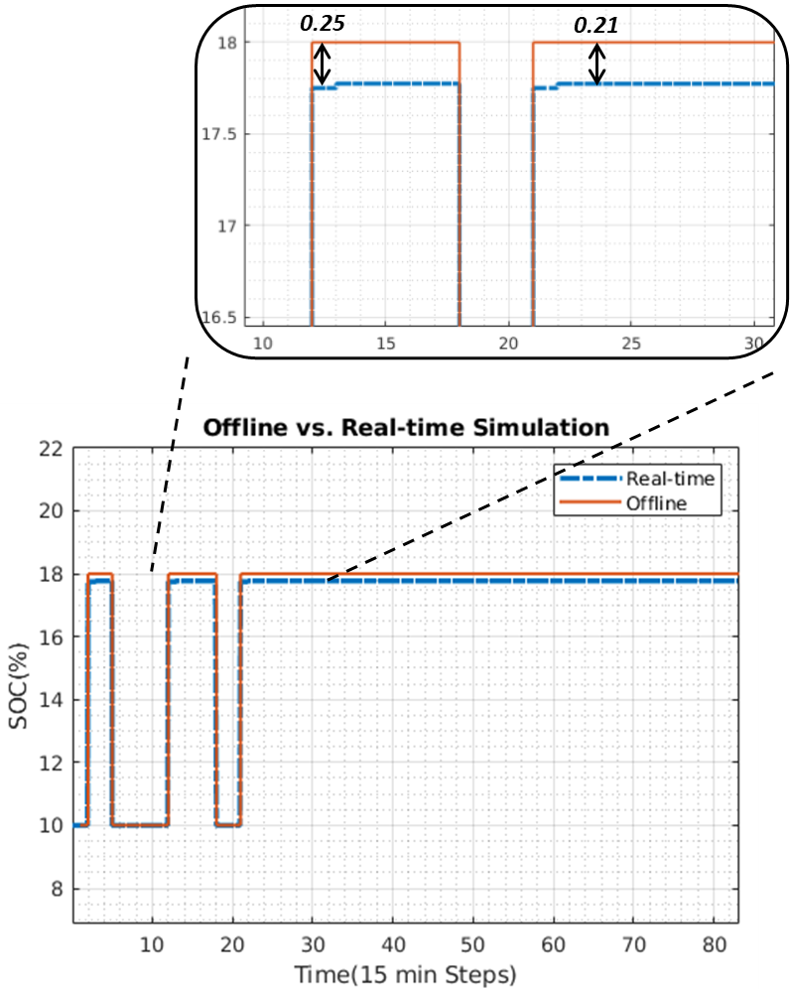
\includegraphics[width = 0.7\linewidth]{figs_juan/realtime.png}
    \caption{State-of-Charge reference for Energy Storage DER in 1-Day Real-time Controller Hardware-in-the-Loop (CHIL) test for Energy Management System.}
    \label{fig:realtime}
\end{figure}

